\documentclass[12pt]{beamer}

\usepackage{thestyle}
\usepackage{thevars}

\begin{document}

  \maketitle

  \begin{frame}{Índice General}
    \setbeamertemplate{section in toc}[sections numbered]
    \tableofcontents[hideallsubsections]
  \end{frame}

  \section{Introducción}

    \begin{frame}[fragile]{Big Data}

      Los algoritmos para \textbf{Big Data} son aquellos que se encargan de resolver problemas sobre conjuntos de datos de tamaño masivo.

    \end{frame}

    \begin{frame}[fragile]{Problema de Accesos a Memoria}

      \begin{figure}
        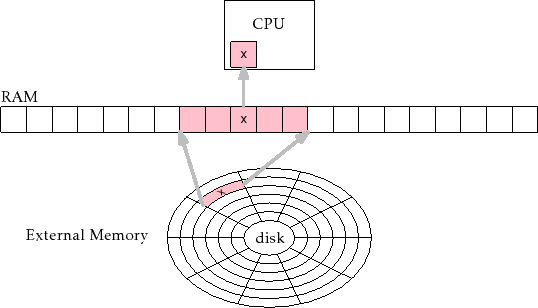
\includegraphics[width=\textwidth,height=0.9\textheight,keepaspectratio]{memory-model}
        \caption{}
        \label{}
      \end{figure}

    \end{frame}

    \begin{frame}[fragile]{Soluciones a la complejidad del Big Data}

      \begin{itemize}
        \item Algoritmos para Streaming
        \item Técnicas de Reducción de la Dimensionalidad
        \item Estrategias de Paralelización
        \item ...
      \end{itemize}

    \end{frame}

  \section{Algoritmos para Streaming}

    \begin{frame}[fragile]{Modelo en Streaming}

    \begin{itemize}
      \item Serie Temporal:\\
        $1, 5, 3, -4, 2, -3, 5,...$
      \item Caja Registradora (Cash-Register): \\
        $(2, +1), (3, +4), (1, +3), (2, +3), (4, +5),...$
      \item Molinete (Turnstile): \\
        $(2, -1), (3, -4), (1, +3), (2, -3), (4, +5),...$
    \end{itemize}

  \end{frame}

    \begin{frame}[fragile]{Algoritmos para Streaming}

      Los \textbf{Algoritmos para Streaming} son aquellos que procesan la entrada de manera secuencial, teniendo en cuenta únicamente el elemento actual, junto con una estimación de los procesados anteriormente, utilizando un orden sublineal $o(n)$ en espacio respecto del rango de posibles valores en la entrada.

    \end{frame}

    \begin{frame}[fragile]{Algoritmos para Streaming}

      \begin{equation}
        F_k = \sum_{i=1}^n m_i^k
      \end{equation}

      \begin{itemize}
        \item Algoritmo de Morris: $F_1$
        \item Algoritmo de Flajolet-Martin: $F_0$
        \item Estimación de Momentos de Frecuencia: $F_k, \ k \in N^*$
      \end{itemize}

    \end{frame}

    \begin{frame}[fragile]{Algoritmo de Flajolet-Martin}

      [TODO ]

    \end{frame}

  \section{Estrategias de Sumarización}

    \begin{frame}[fragile]{Estrategias de Sumarización}

      \begin{itemize}
        \item Muestreo Aleatorio
        \item Histogramas
        \item Wavelets
        \item Sketches
      \end{itemize}

    \end{frame}


    \begin{frame}[fragile]{Sketches}

      \begin{itemize}
        \item Count-Min Sketch
        \item Count Sketch
        \item AMS Sketch
        \item Hyper-LogLog
        \item $L_p$-Samplers
      \end{itemize}

    \end{frame}


    \begin{frame}[fragile]{Count-Min Sketch}

      \begin{figure}
        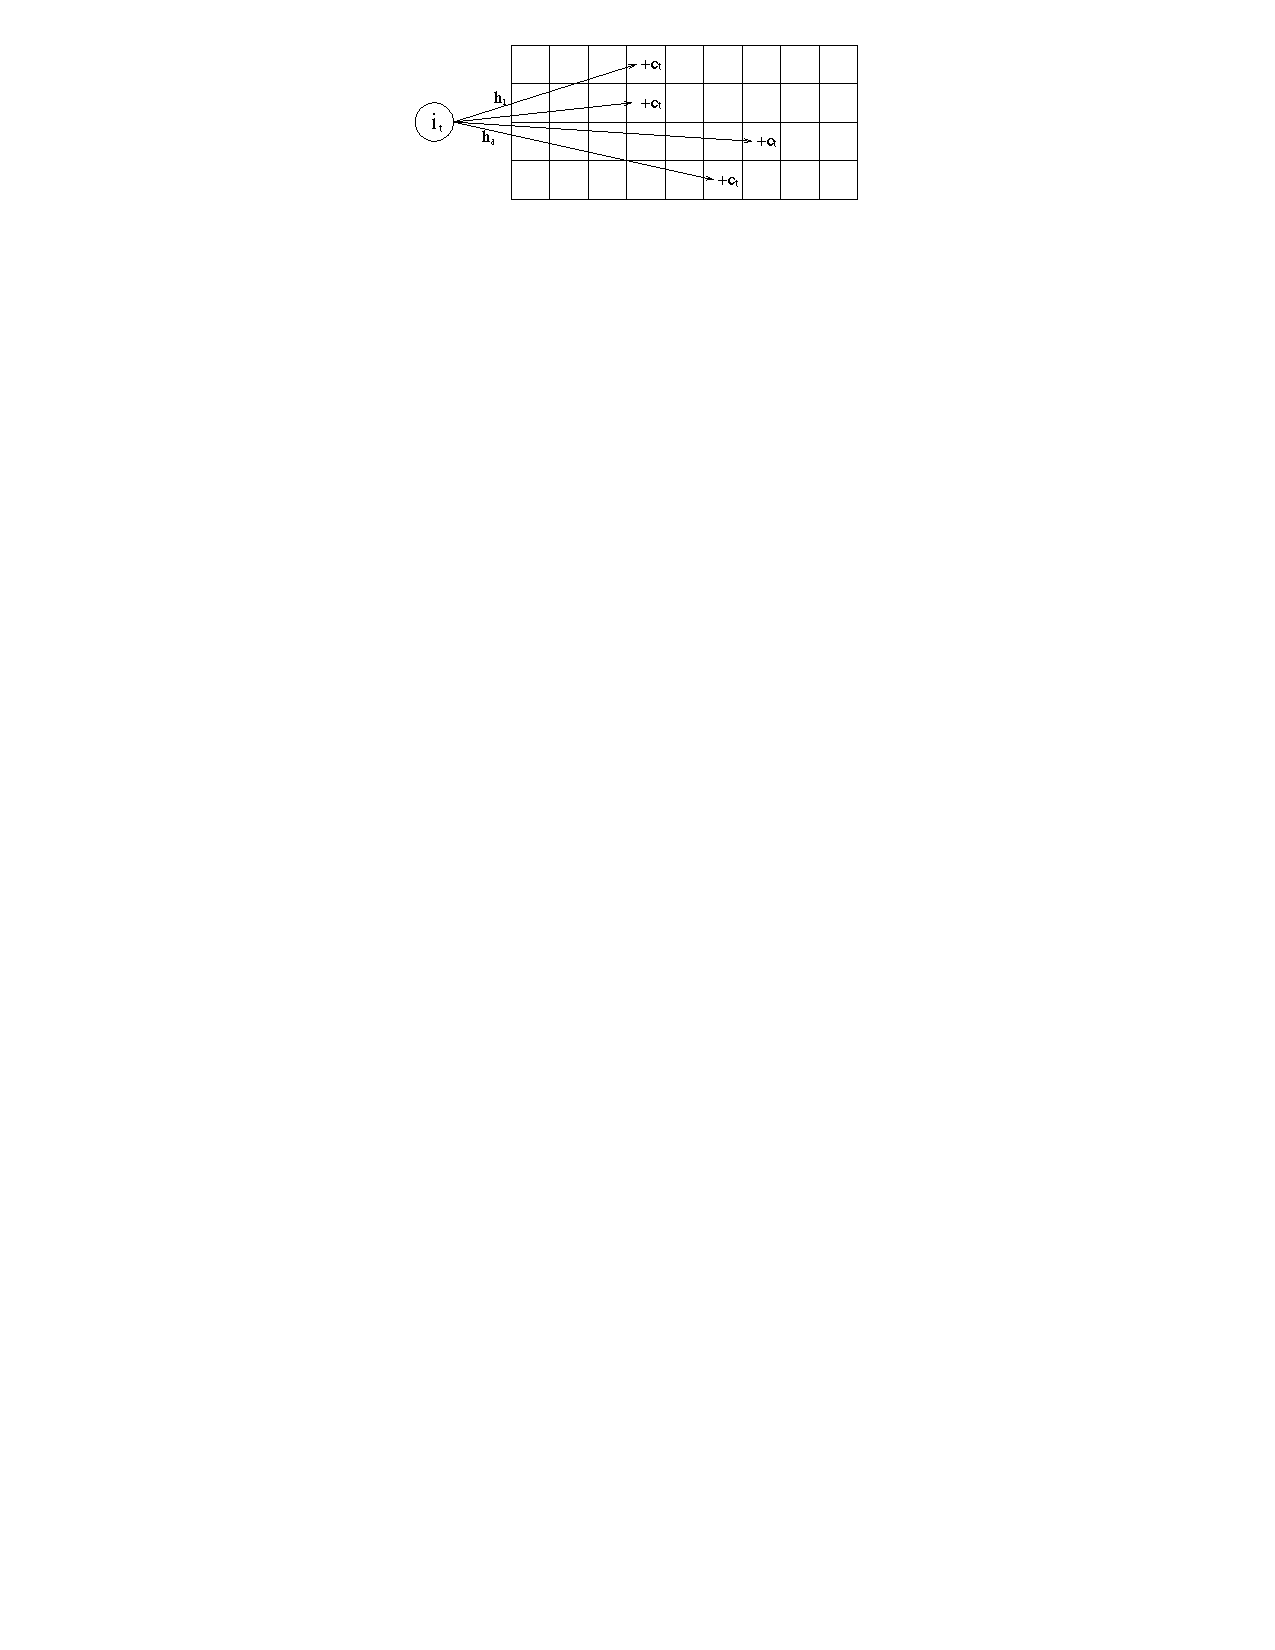
\includegraphics[width=\textwidth,height=0.9\textheight,keepaspectratio]{count-min-sketch}
        \caption{}
        \label{}
      \end{figure}

    \end{frame}

  \section{Algoritmos aplicados a Grafos}

    \begin{frame}[fragile]{Algoritmos aplicados a Grafos}

      Sea $G=(V,E)$ un grafo formado por $n=|V|$ vértices y $m=|E|$ aristas, de tal manera que $e_i = (v_{i_1},v_{i_2}) \in E$ y $\{v_{i_1},v_{i_2}\} \in V$

      Sobre el \textbf{Modelo en Semi-Streaming} se procesa un grafo a través del stream de aristas, en un espacio poli-logarítmico respecto del cardinal de vértices utilizando un número reducido de pasadas sobre el stream.

    \end{frame}

    \begin{frame}[fragile]{Spanners y Sparsifiers}

      \begin{itemize}
        \item Spanner:
        \item Sparsifier:
      \end{itemize}

      \begin{figure}
        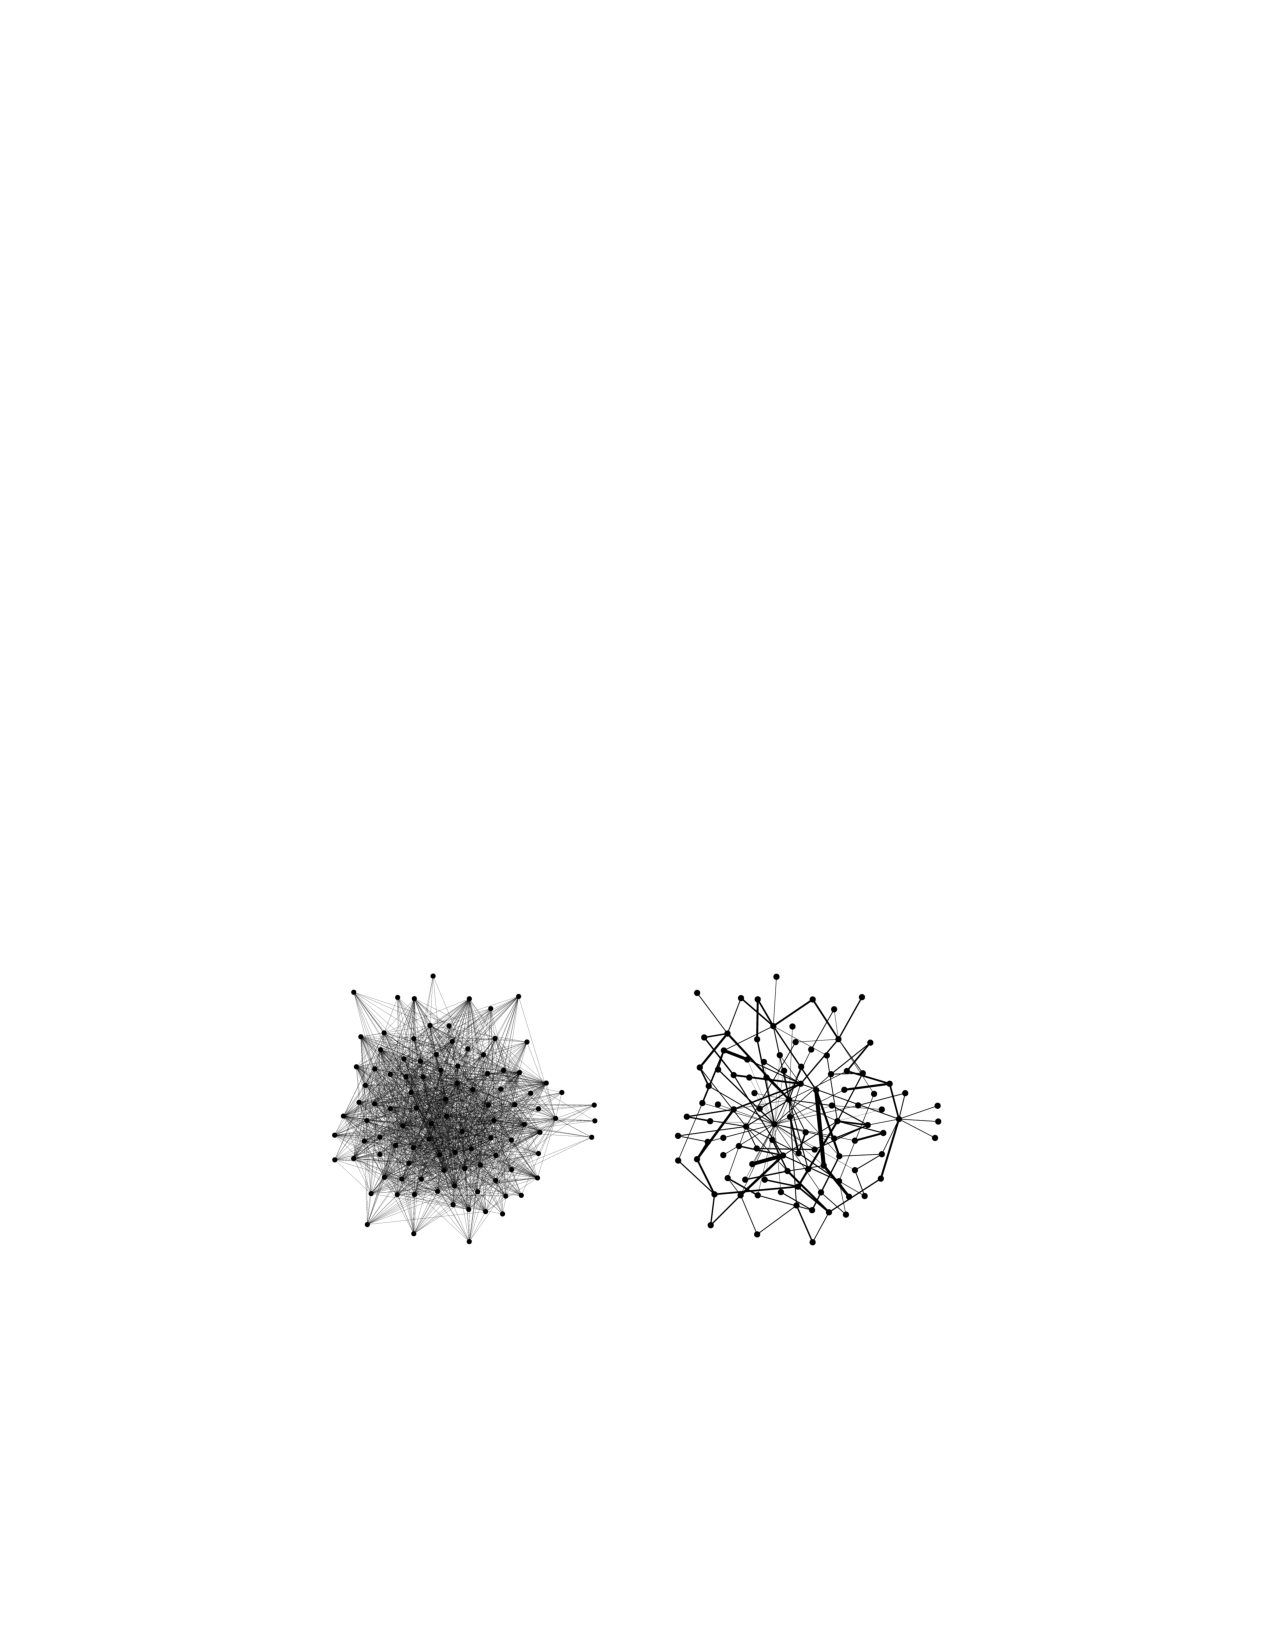
\includegraphics[width=\textwidth,height=0.9\textheight,keepaspectratio]{graph-sparsifier}
        \caption{}
        \label{}
      \end{figure}

    \end{frame}

    \begin{frame}[fragile]{Problemas sobre Grafos}

      \begin{itemize}
        \item Verificación de Grafo Bipartito
        \item Conteo de Triángulos
        \item Árbol Recubridor Mínimo
        \item Componentes Conectados
        \item Paseos Aleatorios
        \item ...
      \end{itemize}

    \end{frame}

  \section{Algoritmo PageRank}

    \begin{frame}[fragile]{Algoritmo PageRank}

      Ranking de los vértices de un grafo basado únicamente en la estructura de relaciones generada por las aristas del grafo.

      Los vértices incidentes con vértices populares tendrán mayor popularidad.

      Distribución estacionaria de la \textbf{Cadena de Markov} subyacente.

    \end{frame}

    \begin{frame}[fragile]{Cadena de Markov}

      \begin{figure}
        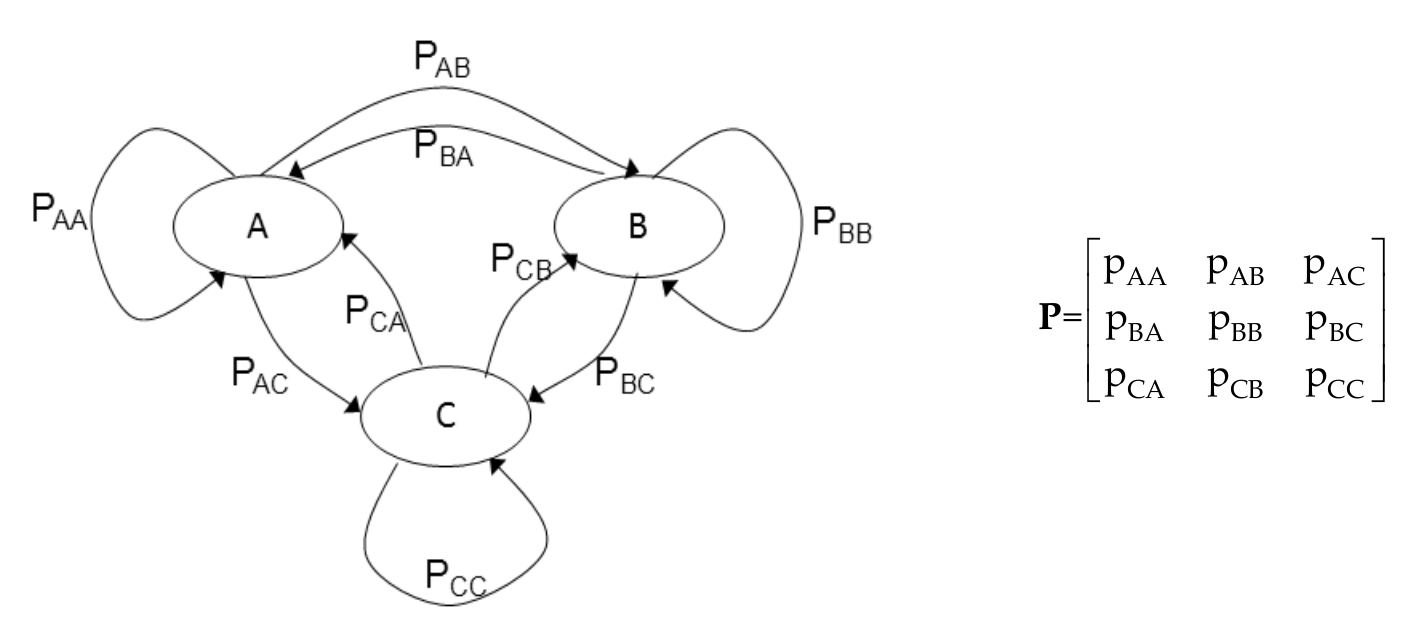
\includegraphics[width=\textwidth,height=0.9\textheight,keepaspectratio]{markov-chain-example}
        \caption{}
        \label{}
      \end{figure}

    \end{frame}

    \begin{frame}[fragile]{PageRank}

      \begin{figure}
        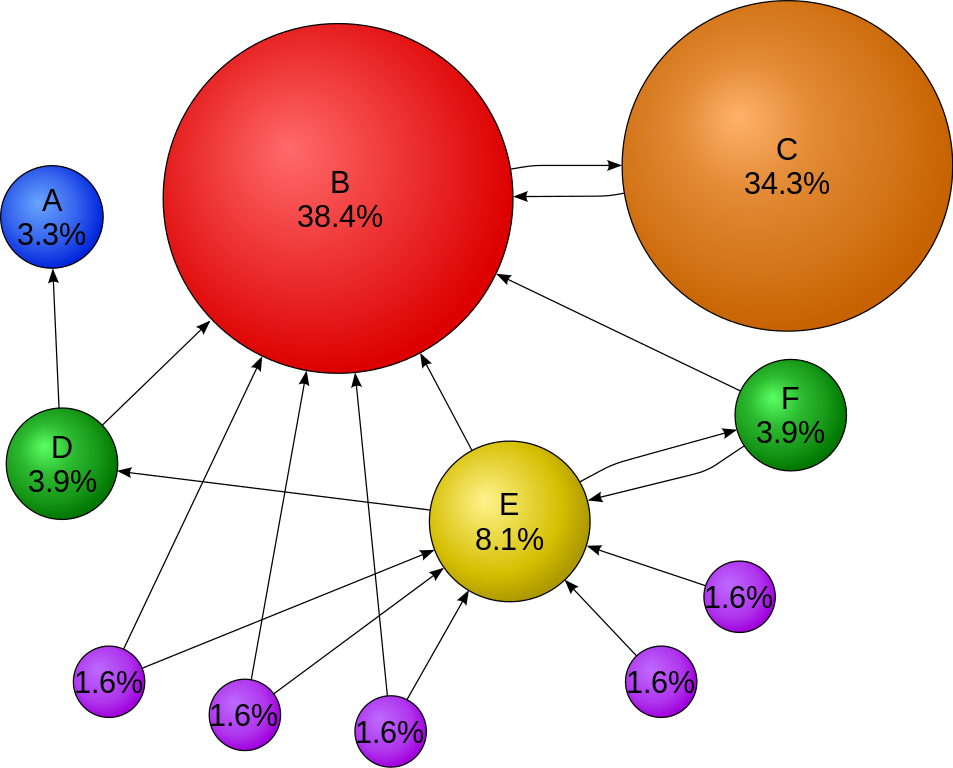
\includegraphics[width=\textwidth,height=0.9\textheight,keepaspectratio]{pagerank}
        \caption{}
        \label{}
      \end{figure}

    \end{frame}

    \begin{frame}[fragile]{Problemas sobre grafos reales}

      \textbf{Vértices Sumidero} no cumplen la propiedad de Cadena de Markov.

      Saltos Aleatorios como solución al problema de los vértices sumidero, siguiendo una distribución uniforme.

    \end{frame}

    \begin{frame}[fragile]{¿Cómo calcularlo?}

      \begin{itemize}
        \item Algebraica [TODO]
        \item Iterativa [TODO]
        \item Paseos Aleatorios
      \end{itemize}

    \end{frame}

    \begin{frame}[fragile]{PageRank Personalizado}

      [TODO ]

    \end{frame}

    \begin{frame}[fragile]{Algoritmos Similares}

      \begin{itemize}
        \item HITS
        \item SALSA
        \item SimRank
      \end{itemize}

    \end{frame}

  \section{Implementación}


    \begin{frame}[fragile]{Implementación}

      La implementación realizada consiste en una biblioteca de grafos (\textbf{tf\_G}) utilizando como base la plataforma de cálculo matemático intesivo \textbf{TensorFlow}.

      \textbf{tf\_G} se encuentra en una fase muy temprana, formando únicamente el conjunto de métodos para el cálculo del \textbf{PageRank}.

    \end{frame}

    \begin{frame}[fragile]{Diagrama de Clases}

      \begin{figure}
        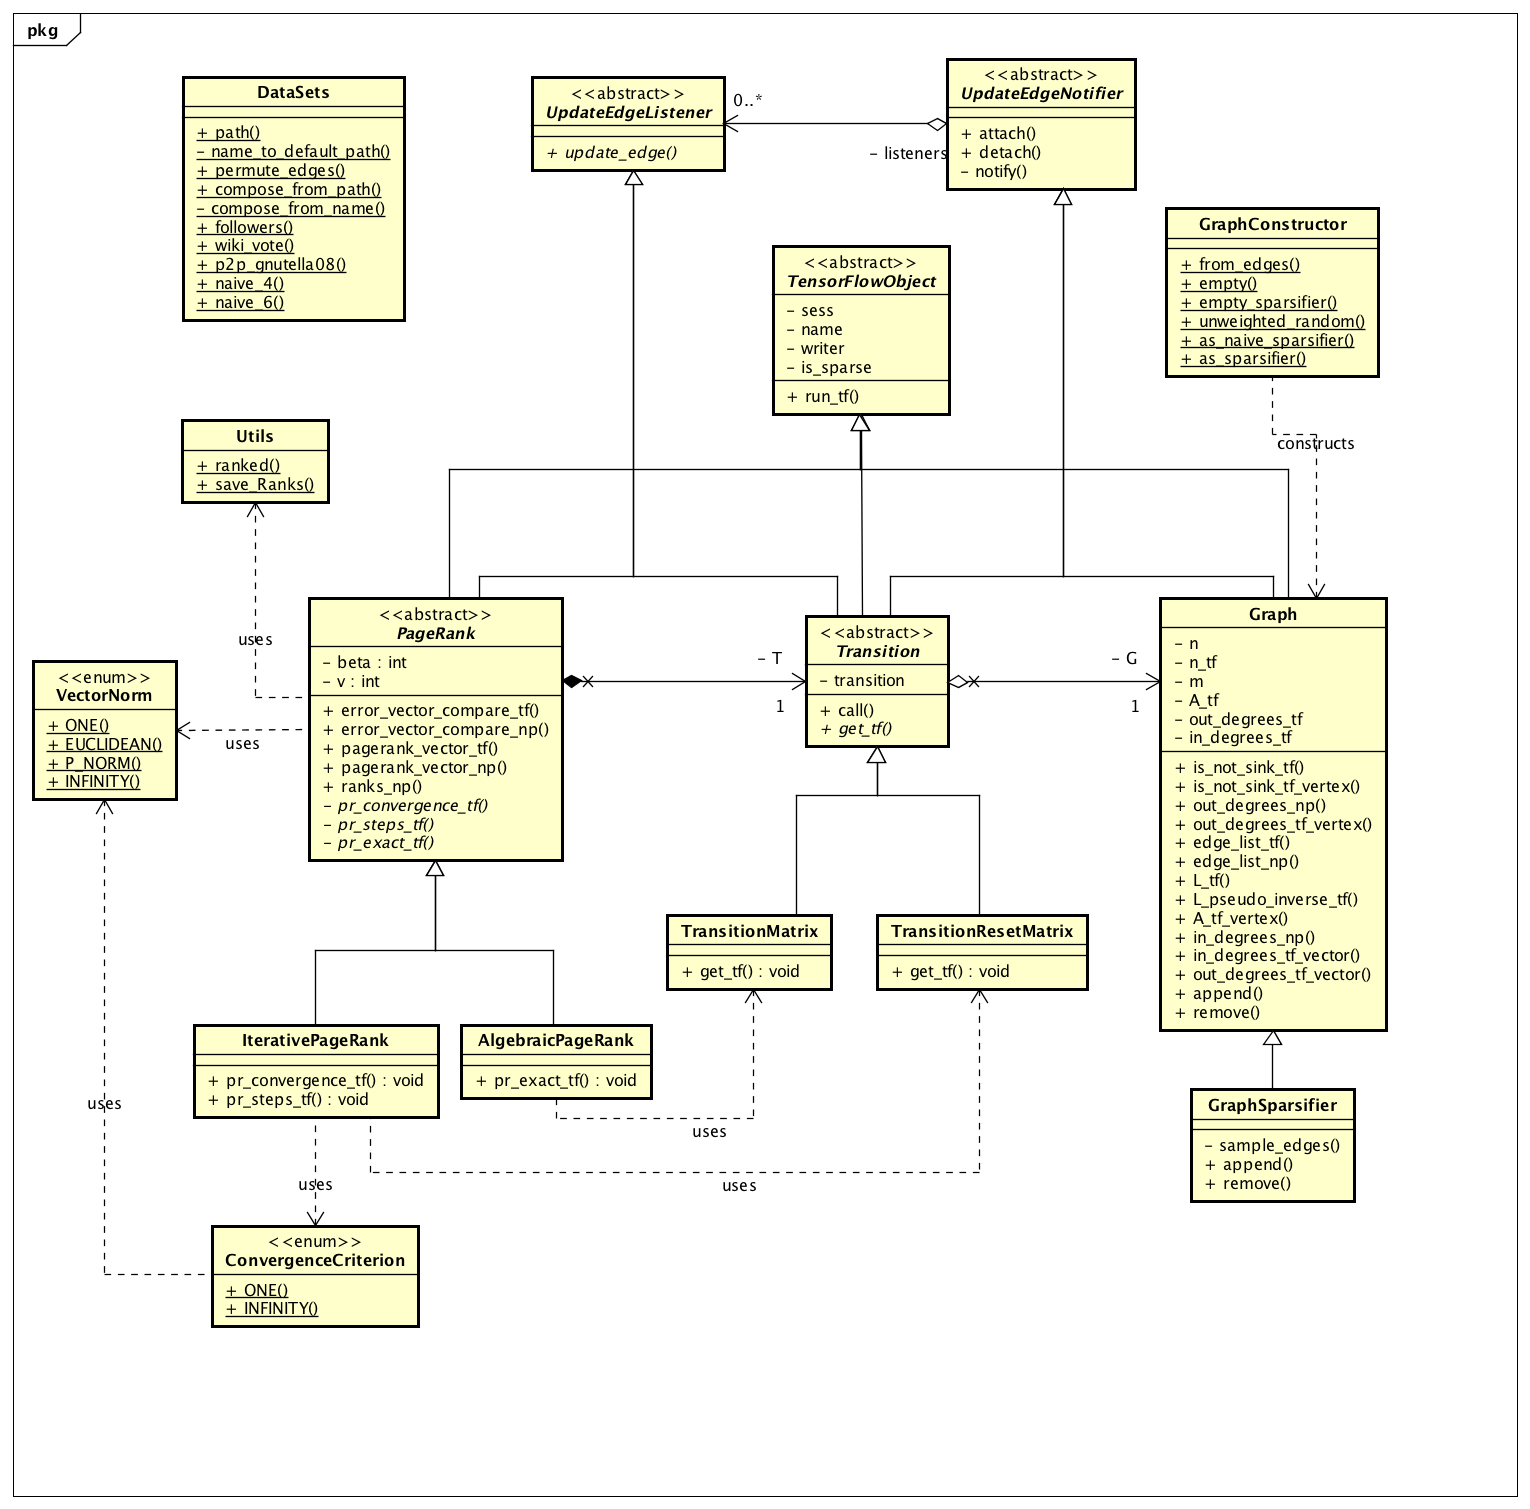
\includegraphics[width=\textwidth,height=0.9\textheight,keepaspectratio]{complete-class-diagram}
        \caption{}
        \label{}
      \end{figure}

    \end{frame}


    \begin{frame}[standout]
      Trabajo completo en: \\
      \small\url{https://github.com/garciparedes/tf_G}
    \end{frame}

  \begin{frame}[standout]
    ¿Preguntas?
  \end{frame}


  \begin{frame}[allowframebreaks]{Referencias}

    \bibliography{bib}
    \bibliographystyle{alpha}

  \end{frame}

\end{document}
